\documentclass[10pt,twocolumn,letterpaper]{article}

\usepackage{cvpr}
\usepackage{times}
\usepackage{epsfig}
\usepackage{graphicx}
\usepackage{amsmath}
\usepackage{amssymb}

% Include other packages here, before hyperref.
\usepackage{algorithm}
\usepackage{algpseudocode}
\usepackage{wrapfig}
\usepackage{subcaption}

\usepackage{caption}
\captionsetup[table]{position=bottom}

\usepackage{array}
\usepackage{epstopdf}
\usepackage{cuted}

% If you comment hyperref and then uncomment it, you should delete
% egpaper.aux before re-running latex.  (Or just hit 'q' on the first latex
% run, let it finish, and you should be clear).
\usepackage[pagebackref=true,breaklinks=true,letterpaper=true,colorlinks,bookmarks=false]{hyperref}

% \cvprfinalcopy % *** Uncomment this line for the final submission

\def\cvprPaperID{****} % *** Enter the CVPR Paper ID here
\def\httilde{\mbox{\tt\raisebox{-.5ex}{\symbol{126}}}}

% Pages are numbered in submission mode, and unnumbered in camera-ready
\ifcvprfinal\pagestyle{empty}\fi

\begingroup
  \catcode`\_=\active
  \gdef_#1{\ensuremath{\sb{\mathrm{#1}}}}
\endgroup
\mathcode`\_=\string"8000
\catcode`\_=12

\usepackage{xcolor}
\usepackage{textcomp}
\definecolor{Gray}{rgb}{0.5,0.5,0.5}
\definecolor{darkblue}{rgb}{0,0,0.7}
\definecolor{orange}{rgb}{1,.5,0} % something readable but different from todo
\definecolor{red}{rgb}{1,0,0} % something readable but different from todo
\newcommand{\heading}[1]{\noindent\textbf{#1}}
\newcommand{\note}[1]{{\em{\textcolor{orange}{#1}}}}
%\newcommand{\todo}[1]{{\textcolor{darkblue}{TODO: #1}}}
\newcommand{\changed}[1]{{\textcolor{blue}{#1}}}

\newcommand{\Matrix}[1]     {{\ensuremath{\mathbf{\uppercase{#1}}}}} %Matrix 
\newcommand{\Vector}[1]     {{\ensuremath{\mathbf{\lowercase{#1}}}}} %Vector
\newcommand{\Variable}[1]   {{\ensuremath{\mathrm{\lowercase{#1}}}}} %Scalar
\newcommand{\Id}            {\mathbb{I}} %Identity matrix

\newcommand{\minimize}[1]   {\underset{{#1}}{\operatorname{argmin}} \: \: } %Minimize w.r.t.
\newcommand{\subjectto}     {\operatorname{subject to}}

\newcommand{\signal} {\Vector{x}}
\newcommand{\filter} {\Vector{d}}
\newcommand{\code}   {\Vector{z}}
\newcommand{\Filter} {\Matrix{D}}
\newcommand{\mask}   {\Matrix{M}}
\newcommand{\Code}   {\Matrix{z}}
\newcommand{\surC}   {\Matrix{C}}
\newcommand{\surB}   {\Matrix{B}}


\begin{document}

%%%%%%%%% TITLE
\title{Stochastic Convolutional Sparse Coding}

\author{First Author\\
Institution1\\
Institution1 address\\
{\tt\small firstauthor@i1.org}
% For a paper whose authors are all at the same institution,
% omit the following lines up until the closing ``}''.
% Additional authors and addresses can be added with ``\and'',
% just like the second author.
% To save space, use either the email address or home page, not both
\and
Second Author\\
Institution2\\
First line of institution2 address\\
{\tt\small secondauthor@i2.org}
}

\maketitle
%\thispagestyle{empty}

%%%%%%%%% ABSTRACT
\begin{abstract}
The minimization problems formulated in Convolutional Sparse Coding (CSC) have been solved in frequency domain by modern approaches owing to the improved computing efficiency. However, solving the problem in frequency domain automatically assumes circular boundary conditions, and also it is restricted by imposing modern optimization strategies for this specific problem. In this work, we propose a novel stochastic spatial-domain solver, in which a randomized subsampling strategy is introduced in the subproblem of computing sparse codes. Afterwards, we extend the proposed strategy in conjunction with online learning, scaling the CSC model up to arbitrary sample sizes. In both cases, we show experimentally that the proposed method, with a reasonable selection of the subsampling rate, outperforms the state-of-the-art frequency-domain solvers in terms of execution time without losing the learning quality. At last, we evaluate the effectiveness of the over-complete dictionary learned from large-scale datasets that has not been studied by precedent CSC work, which demonstrates an improved sparse representation of the natural images on account of more abundant learned image features.
\end{abstract}

%%%%%%%%% BODY TEXT
\section{Introduction}
Convolutional Sparse Coding (CSC) is a method for learning {\em
  generative} models in the form of translationally invariant
dictionaries for a large variety of different training signals.  These
generative models have been shown effective for solving problems in
neural and brain information
processing~\cite{jas2017learning,peter2017sparse}, as well as in a
variety of image processing tasks, for instance, image
inpainting~\cite{heide2015fast},
super-resolution~\cite{gu2015convolutional}, high dynamic range
imaging~\cite{serrano2016convolutional}, and high-dimensional signal
reconstructions~\cite{choudhury2017consensus,bibi2017high}. CSC
differs from conventional sparse coding by formulating the signals as
the sum of a set of convolutions on dictionary filters and sparse
codes instead of patch-wise linear combinations of
filters. In traditional sparse dictionary learning, the patch
structure significantly degrades the expressiveness of the
dictionaries by introducing a strong dependency on the position of a
feature, which the convolutional nature of CSC avoids.
%% Alternatively, sparse coding, as a patch-based approach,              %%
%% learns filters from partitioned local structures, and this partition  %%
%% manipulation discards inherent correlations between those patches, so %%
%% as to learns redundant filters (the same or similar ones with         %%
%% translated versions). Owing to the convolutional property, the        %%
%% dictionary learned from CSC achieves signal global coherence, tending %%
%% to be more representative.                                            %%

Of course this convolutional approach is also a the heart of many deep
learning-based methods in the form of
CNNs~\cite{lecun1998gradient,kavukcuoglu2010learning,krizhevsky2012imagenet},
which have in recent years been extraordinarily successful for a broad
range of high-level image understanding applications. However, while
CNNs generally are used in a {\em supervised} setting and produce {\em
  discriminative}, task-specific models, CSC is {\em unsupervised} and
produces {\em generative} models that easily transfer between tasks.

To solve the optimization problems inherent to CSC, Zeiler et
al.~\cite{zeiler2010deconvolutional} iteratively solve two subproblems
(updating sparse codes and updating filters) using gradient decent in
the form of convolutional operations in the spatial domain, which is
computationally expensive. Recent algorithms tackle the problem by
exploiting Parseval's theorem to express the spatial convolution by
multiplication in the frequency domain and using proximal solver such
as Alternating Direction Method of Multipliers
(ADMM)~\cite{boyd2011distributed} to separate the linear least squares
parts terms from the non-smooth terms in the optimization
problem. These approaches show tremendous improvements over prior
spatial-domain solvers with respect to running
time~\cite{bristow2013fast,heide2015fast,wohlberg2016efficient,choudhury2017consensus}. Most
of the prior work learns the dictionary filters in a batch mode, which
indicates that all training signals are involved in every training
iteration, and this restricts it from applying to large datasets or
streaming data.

In contrast to batch mode learning, online
learning~\cite{shalev2012online} is a well established strategy which
processes a single image or a small portion (mini-batch) of the whole
data at each training step, and incrementally updates model
variables. Herein, the required memory and computing sources are only
dependent on the sample size in every observation, independent of the
training data size. It alleviates the scalability issue that arises in
batch approaches, and the convergence of the algorithm was firstly
analyzed using stochastic approximation
tools~\cite{bottou1998online}. Bottou et
al.~\cite{bousquet2008tradeoffs} further showed better generalization
performance of the stochastic algorithms than standard gradient
descent on large scale learning systems. Later on, online learning
strategies were synergetic with sparse coding, which was then scaled
up for learning dictionary from millions of training
samples~\cite{mairal2009online,mairal2010online}, and for large-scale
matrix factorization with an additionally introduced subsampling
strategy~\cite{mensch2016dictionary}. More recently, Liu et
al.~\cite{liu-2018-first} and Wang et al.~\cite{wang2018scalable}
separately proposed similar online learning frameworks for the CSC
model, alleviating the memory issues arise in batch-based CSC model on
large datasets.

{\bfseries Contributions.} We mainly make three contributions in this
work. First, we introduce a randomization strategy for the CSC
model and solve the entire problems in spatial domain. We demonstrate
that the proposed stochastic spatial-domain solver, with a reasonably
selected subsampling rate, outperforms the state-of-the-art
frequency-domain solvers with regard to computing efficiency. We then
formulate an online-learning version of the proposed algorithm, and 
show dramatic runtime improvement over current online CSC methods,
while producing comparable outcomes. Finally, we demonstrate the
capability to learn the over-complete dictionary from thousands of
images, and analyze the effectiveness of the learned over-complete
dictionary for a number of reconstruction tasks.


% --- DO NOT DELETE ---
% Local Variables:
% mode: latex
% mode: flyspell
% mode: TeX-PDF
% End:



\section{Convolutional Sparse Coding (CSC)}
Specifically, the CSC problem is trying to minimize
\begin{equation}
\begin{split}
    \minimize{\filter,\code} & \frac{1}{2}\|\signal - \sum_{k=1}^{K} \filter_k * \code_k \|_2^2 + \lambda \sum_{k=1}^{K}\| \code_k \|_1 \\
    \subjectto & ~ \|\filter_k\|^2_2 \leq 1 ~~ \forall k \in {1,...K},
\end{split}
\end{equation}
where $\signal \in \mathbb{R}^D$ is a D-dimensional signal or a vectorized image~\footnote{In this manuscript, we work on 2D images.}, $\filter_k \in \mathbb{R}^M$ is the $k$-th dictionary and $\code_k$ is the sparse code associated with that dictionary, and it has the same dimension size as $\signal$. $K$ is the number of dictionary filters, and $*$ is the convolution operator. The above equations will be applied to all the training images.

The modern approaches exploit Parseval's theorem and introduce two slack variables to separate the non-smooth $L_1$ penalty term and the $L_2$ constraints, making it feasible to be efficiently computed in frequency domain, and to apply splitting strategy to formulate the problem into ADMM framework, where the two subproblems (updating $\code$ and updating $\filter$) are jointly solved by coordinate descent~\cite{bristow2013fast,heide2015fast,wohlberg2016efficient}. There exists several common issues regarding to the model and the frequency solvers.

\begin{itemize}
  \item Though CSC overcomes the independence assumption held in patch-based learning algorithms, far more variables ($K$ times more), as a payback, will be introduced to represent a single image. This brings in more severe memory and computational burden.
  \item The reconstructed sparse codes show that in the case of $K=100$, the majority of the entries (more than $99.5\%$) do not provide valid information to the represented image, which indicates the subproblem for updating $\code$ solves a highly sparse LASSO problem. Transforming the problem into frequency domain imposes restriction on the use of optimization strategies for this very specific problem.
  \item The prior work shows its efficiency of solving the CSC problem in frequency domain, while this is only applicable for updating $\code$, and it does not hold for updating $\filter$. The dictionary filters usually have much smaller spatial support than the dimension size of the sparse codes ($M \ll D$), while in order to tackle the problem in frequency domain, it requires to process the $\filter$-subproblem in the same dimensions as the sparse codes, and then project the results onto its small spatial support.
\end{itemize}

\section{Stochastic Convolutional Sparse Coding}
\subsection{The Model}
Since the images are represented by a set of highly sparse codes, we have observed that they can be well reconstructed by a random subset of the sparse codes. Based on this observation, we propose a variant of the $\code$-subproblem using subsampling strategy, and formulate the following modified minimization problem:
\begin{equation} \label{eq:updatingCode}
    \minimize{\code} \frac{1}{2}\|\signal - (\Filter \mask^T)(\mask \code) \|_2^2 + \lambda \|\mask \code\|_1,
\end{equation}
where $\Filter = [\Filter_1 ... \Filter_K] \in \mathbb{R}^{D \times DK}$, $\code = [\code_1^T ... \code_K^T]^T \in \mathbb{R}^{DK \times 1}$, the convolution operator are formulated in matrix multiplication so that $ \Filter \code = \sum_{k=1}^{K} \filter_k * \code_k$.  $\mask$ is a randomized sub-sampling diagonal matrix with $1$ on the entries corresponding to the sampled sparse codes, performing the function of choosing a random portion of the sparse codes for reconstruction. Herein, the $\code$-subproblem only computes the sparse codes in the chosen positions. Due to the introduced subsampling matrix, the convolution operator will not hold, hence it cannot be solved in the frequency domain. This subsampling strategy is akin to the dropout technique~\cite{srivastava2014dropout}, which has been widely used to prevent overfitting when training deep neural networks. However, different from dropout that generally needs more time to train a neural network than standard approaches, with a good selection of subsampling probability $p$, the proposed method shows less per iteration running time and faster convergence than state-of-the-arts (see section~\ref{sec:result}).

After obtaining the subsampled codes, we can then project them onto its original spatial support with $0$ filling. Afterwards, the dictionary can be updated by:
\begin{equation} \label{eq:updatingFilter}
    \minimize{\filter} \frac{1}{2}\|\signal - \Code \filter \|_2^2, ~\subjectto ~ \|\filter_k\|^2_2 \leq 1 ~ \forall k \in {1,...K},
\end{equation}
where $\Code= [\Code_1 ... \Code_K] \in \mathbb{R}^{D \times MK}$ and $\filter= [\filter_1^T ... \filter_K^T]^T \in \mathbb{R}^{MK \times 1}$ such that $ \Code \filter = \sum_{k=1}^{K} \filter_k * \code_k$.

Like the approach in~\cite{heide2015fast}, we interleave on the above two subproblems to tackle the bi-convex problem, and each of them will be solved by ADMM. The jointly optimization framework will be implemented in the fashions of batch mode and online mode.

\begin{minipage}[t]{0.5\textwidth}
\vspace{0pt}
\begin{algorithm}[H]
\caption{SBCSC} \label{algo:SBCSC}
\begin{algorithmic}[1]
\State $\text{Initialize} ~ \filter;$
\While {not converge}
    \State $\Filter \gets \text{constructD}(\filter);$
    \For{i=1 to N}
        \State $ \text{Generate } \mask \text{ given } p;$
        \State $ \text{Update } \code^i \text{ by solving problem~\ref{eq:updatingCode}};$
    \EndFor
    \State $\Code \gets \text{constructZ}(\code^{1,...,N});$
    \State $\text{Update } \filter \text{ by solving problem~\ref{eq:updatingFilter}} ;$
\EndWhile
\end{algorithmic}
\end{algorithm}
\end{minipage}
\begin{minipage}[t]{0.5\textwidth}
\vspace{0pt}
\begin{algorithm}[H]
\caption{SOCSC} \label{algo:SOCSC}
\begin{algorithmic}[1]
\State $\text{Initialize} ~ t=0, \filter^t,  \surC^t = 0, \surB^t = 0$
\While {not converge}
    \State $\Filter \gets \text{constructD}(\filter^t);$
    \State $t \gets t+1$
    \State draw($\signal^t$, $\mask$);
    \State $ \text{Compute } \code^t \text{ by solving problem~\ref{eq:updatingCodeOnline}};$
    \State $\Code \gets \text{constructZ}(\code^t)$
    \State Compute $\surC^t$ and $\surB^t$ by eq~\ref{eq:updateSur}
    \State Update $\filter^t$ by solving problem~\ref{eq:updatingFilterOnline}
\EndWhile
\end{algorithmic}
\end{algorithm}
\end{minipage}

\subsection{Stochastic Batch CSC (SBCSC)}
We first formulate the batch-mode of the proposed method as shown in Algorithm~\ref{algo:SBCSC}, where $N$ is the number of total input images, $\code^i$ is the sparse code associated with $i$-th image, and $p$ is the probability for one specific code been selected. Every outer loop involves all of the training images, thus it would be expensive in computing these and also runs out of memory quickly with the increase of the number of images. The batch-based learning algorithm lacks of the capability to scale up to very large datasets or to handle dynamically changed training data.

\subsection{Stochastic Online CSC (SOCSC)}
We can further tackle the proposed problem in online fashion for a gain of scalability. In the online learning setting, each iteration only draws one or a subset (minibatch) of the total training images, hence the complexity per loop is independent of the training sample size. Then, given the sampled image $\signal^t$ at $t$-th iteration, we can compute the corresponding sparse codes $\code^t$ by
\begin{equation} \label{eq:updatingCodeOnline}
    \code^t = \minimize{\code} \frac{1}{2}\|\signal^t - (\Filter^{t-1} \mask^T)(\mask \code) \|_2^2 + \lambda \|\mask \code\|_1,
\end{equation}
where $\Filter^{t-1}$ is constructed from the dictionaries learned by $(t-1)$th iteration. After obtaining the sparse codes, the dictionary is updated by:
\begin{equation}
    \filter^t = \minimize{\filter} \frac{1}{2t}\sum_{i=1}^{t} \|\signal^i - \Code^i \filter \|_2^2, ~\subjectto ~ \|\filter_k\|^2_2 \leq 1 ~ \forall k \in {1,...K}.
\end{equation}
Notice that updating dictionary involves all the past training images and sparse codes. As shown in~\cite{mairal2009online,mairal2010online}, we can get rid of explicitly storing those data by introducing two surrogate matrices $\surC \in \mathbb{R}^{KM \times KM}$ and $\surB \in \mathbb{R}^{KM \times 1}$, which carry all of the required information for updating $\filter$, and can be iteratively updated by:
\begin{equation} \label{eq:updateSur}
    \surC^t  = \frac{t-1}{t} \surC^{t-1} + \frac{1}{t}(\Code^t)^T\Code^t ~~~~~~~~~ \surC^t  = \frac{t-1}{t} \surB^{t-1} + \frac{1}{t}(\Code^t)^T\signal^t
\end{equation}
If so, the updated dictionary can be obtained by solving:
\begin{equation} \label{eq:updatingFilterOnline}
    \filter^t = \minimize{\filter} \frac{1}{2} \filter^T\surC\filter - \filter^T\surB, ~ \subjectto ~ \|\filter_k\|_2^2 \leq 1 ~ \forall k \in {1,...K}
\end{equation}

\subsection{Implementation Details}
Updating $\code$ in Algorithm\ref{algo:SBCSC} (Problem~\ref{eq:updatingCode}) is the standard LASSO, and we solve it by well-known ADMM framework. The data fitting term and the $L_1$ penalty term are split, forming $x$-minimization step and $z$-minimization step, respectively. $x$-minimization step is a quadratic programming (QP) problem, and we cache the matrix factorization by Cholesky decomposition. $z$-minimization step can be solved by a point-wise shrinkage operation. Accordingly, updating $\filter$ (problem~\ref{eq:updatingFilter}) is a quadratic constrained quadratic programming (QCQP) problem, and we solve it using similar splitting and optimization strategies as solving Problem~\ref{eq:updatingCode}, except using Conjugate Gradient (CG) for $x$-minimization step and replacing the shrinkage function by projecting onto the constrained set for $z$-minimization step. The $\filter$-subproblem is warm started with previously computed results and these two subproblems are interleaved on their auxiliary variables. The corresponding subproblems in Algorithm~\ref{algo:SOCSC} are solved following the same optimization strategy as discussed above. We set the hyperparameters $\lambda=1$,  the augmented Lagrangian penalty $\rho_{\code}$ and $\rho_{\filter}$ to $10 \lambda$ and $50 \lambda$, respectively, for $\code$- and $\filter$-subroblem. The ADMM iteration is fixed to 10 for all subroutines, and the over-relaxation strategy within ADMM is applied with $\alpha = 1.8$. The residual tolerance for CG is $1e^{-5}$.

All the training and evaluation processes in this manuscript are performed on contrast normalized images. %We also tried to learning filters from images without pre-processing with little parameters tuning, which successfully learns similar Gabor-like features as learned from contrast normalized images, as well as low frequency filters. The results regarding to this will not be discussed in this work, while it can be applied to other applications where low frequency parts also need to be taken into account. %
It should be noted that matrix $\Code$ needs to be explicitly constructed and it may lead to a considerable computational burden, resulting in a heavy overhead if processed in an inefficient way. In our implementation, the vector-to-matrix mapping information is cached for an efficient indexing. As for matrix $\Filter$, we only explicitly construct matrix $(\Filter \mask^T)$ rather than $\Filter$ and $\mask$ separately for the sake of efficiency, and the similar indexing strategy is applied.

\section{Results} \label{sec:result}
\subsection{Sub-Sampling Strategy}
We first evaluate the convergence and effectiveness of the proposed sub-sampling strategy, and compare it with state-of-the-art frequency solver~\cite{heide2015fast}. The proposed algorithm, with different sub-sampling factors, was tested on the fruit dataset~\cite{zeiler2010deconvolutional} which contains 10 training images in the size of $100 \times 100$. The dictionary dimension size is set to $11 \times 11 \times 100$.

{\bfseries Convergence.} Comparisons of the convergence between the proposed method and the state-of-the-art are shown in Fig.~\ref{fig:subsampleResult}. A different selection of the subsampling probability reveals that the proposed strategy will slightly influence the convergence and the training objective of the minimization problem. Specifically, the more subsampled, the relatively slower convergence and the higher objective will be obtained. On the other hand, small subsampling rate will significantly accelerate the computation process, where $10\%$ subsampling achieves about $6 \times$ speedup over no subsampled solver and $2 \times$ speedup over state-of-the-art frequency solvers for one iteration. We observe that a subsampling rate between $0.1$ and $0.2$ delivers empirically good enough convergence in our settings, as well as achieving at least $3 \times$ speedup. It should be clarified that for a better representation, the cropped objectives are plotted after the first iteration, while all of them have the same initial objective. Notice that the comparable method has a relatively high objective at first $6-8$ iterations due to different splitting strategies are applied and subproblems are interleaved on the primary variables~\cite{wohlberg2016efficient}, though it converges to an optimum with comparable objective after 10 iterations. In summary, comparing to the state-of-the-art frequency solver, the proposed method with a subsampling rate of $10\%$ not only spends two times less processing time per iteration, but also needs fewer iterations to converge.

\begin{figure}[h]
\begin{subfigure}{0.6\textwidth}
  \includegraphics[width=1\linewidth]{figure/iteVSobj.pdf}
\end{subfigure} 
\begin{subfigure}{0.3\textwidth}
  \includegraphics[width=1\linewidth]{figure/batchFruit100.pdf}
\end{subfigure}

\begin{subfigure}{0.6\textwidth}
  \includegraphics[width=1\linewidth]{figure/timeVSobj.pdf}
\end{subfigure}
\begin{subfigure}{0.3\textwidth}
  \includegraphics[width=1\linewidth]{figure/heideFruit100.pdf}
\end{subfigure}

\caption{Left: Convergence comparison between the-state-of-art method\cite{heide2015fast} and the proposed method with different subsampling probability. Right: Learned filters by the proposed method with $p=0.1$ and the comparable method. In these represented learned filters, our method learns more Gabor-like and less noise-like filters. Beyond this, it runs faster with regard to each iteration and shows better convergence behavior.}
\label{fig:subsampleResult}
\end{figure}

{\bfseries Reconstruction}. The learned filters by the proposed method with subsampling rate $0.1$ are shown on the right hand side of Fig.~\ref{fig:subsampleResult}. For a visual comparison, we also show the filters learned from the competing method. As can be observed, both of them learn some seemingly similar Gabor-like filters. While after zooming, it can be seen that our learned Gabor-like filters have less impure structures. Moreover, the comparable filters contain a number of noise-like dictionaries, which are rarely existed in ours. We then demonstrate the effectiveness of the reconstructed filters in the application of image inpainting, which refers to reconstructing a full image from partial measurements. A numerical comparison of the reconstruction quality is shown in Fig.~\ref{fig:PSNRrecon}. The filters learned by the proposed method not only show more visually decent structures and less specific features, but also demonstrate its capability to better reconstruct partial observed images. In addition to that, the learning process only takes about $40\%$ of the execution time of the comparison.

\begin{figure}[h]
    \includegraphics[width=1\textwidth]{figure/reconImage.pdf}
    \\
    \resizebox{1\linewidth}{!}{
        \begin{tabular}{|c||c|c|c|c|c|c|c|c|c|c|}
            \cline{1-11}
            Image & 1 & 2 & 3 & 4 & 5 & 6 & 7 & 8 & 9 & 10 \\
            \hline
            PSNR~\cite{heide2015fast} & 25.77 & 24.67 & 24.89 & 23.88 & 24.68 & 25.26  & 24.15 & 25.75 & 22.97 & 26.16 \\
            \hline
            PSNR ours & \textbf{25.91} & \textbf{24.72} & \textbf{25.21} & \textbf{24.09} & \textbf{25.00} & \textbf{25.36} & \textbf{24.32} & \textbf{25.80} & \textbf{23.24} & \textbf{26.37} \\
            \hline
        \end{tabular} }
    \caption{Numerical comparisons of the reconstruction quality obtained from the presented filters and its comparison. The reconstructions are performed on $20\%$ randomly observed images, with $\lambda = 0.4$ and $50$ ADMM iterations for both cases. Obtained PSNR values are averaged on 5 trials. Note that none of the testing images are in the training sets.} \label{fig:PSNRrecon}
\end{figure}

\subsection{Online Learning Settings}
We further evaluate the online fashion of the proposed method. To begin with, we validate the proposed algorithm on the city dataset~\citep{zeiler2010deconvolutional}, which has 10 training images and 4 testing images, and all of them has the size of $100 \times 100$. Afterwards, we analyze the effectiveness of over-complete dictionary learned from 1000 images randomly picked up from ImageNet~\cite{deng2009imagenet}.

{\bfseries Convergence.} Unlike the batch-based learning approaches, the training loss objective of the entire dataset cannot be evaluated since each training step only draws one or a few of the data samples. Otherwise, we can evaluate the learning process on testing images. The loss objectives on testing dataset of the proposed algorithm and prior published online CSC model solved in frequency domain~\citep{liu-2018-first}, with respect to iterations, are shown in Fig.~\ref{fig:onlineSmall}. In the same figure, we also keep track of the capability of the updated filters in the learning process to sparsely represent the testing images, which are demonstrated by its PSNR. These two approaches stop at optimum positions with close testing objective values, though, they exhibit slightly different convergence behaviors with respect to iterations. The final testing PSNR values for both methods also reveal the similar reconstruction performance of the learned filters. As for the runtime comparison, the proposed method runs at least 5 times faster than its comparative.

%The proposed method not only exhibits a better convergence performance, but also takes much less execution time, achieving roughly $5 \times$ speedup for one iteration. A visual comparison of the learned dictionaries also demonstrates that the proposed algorithm delivers better outcomes. 
% Further numerical comparison will be reported in the next section.

\begin{figure}[h]
\centering
\begin{subfigure}{0.45\textwidth}
  \includegraphics[width=1\linewidth]{figure/onlineVSliu-ite.pdf}
\end{subfigure} 
\begin{subfigure}{0.45\textwidth}
  \includegraphics[width=1\linewidth]{figure/onlineVSliu-time.pdf}
\end{subfigure}

\caption{Left: Convergence of the test set objectives for the proposed method and its comparison~\cite{liu-2018-first}. Right: Testing PSNR with respect to execution time. Our method has the similar outcomes as the comparable method, while it achieves $5 \times$ speedup. }
\label{fig:onlineSmall}
\end{figure}

{\bfseries Over-complete dictionaries.} As far as we know, none of the precedent CSC work reported or analyzed the over-complete dictionary (the number of filters is more than the degrees of freedom). One of the reasons could be that most of the prior work is batch-based approach, thus learning over-complete dictionary from small dataset would cause the overfitting issue, which may contain quite a few data-specific filters, and therefore be short of the generalization ability. The proposed online-based learning strategy can overcome this issue by scaling up to arbitrary sample sizes.

\begin{figure}[h]
\begin{minipage}{0.4\textwidth}
\begin{subfigure}{1\textwidth}
    \centering
  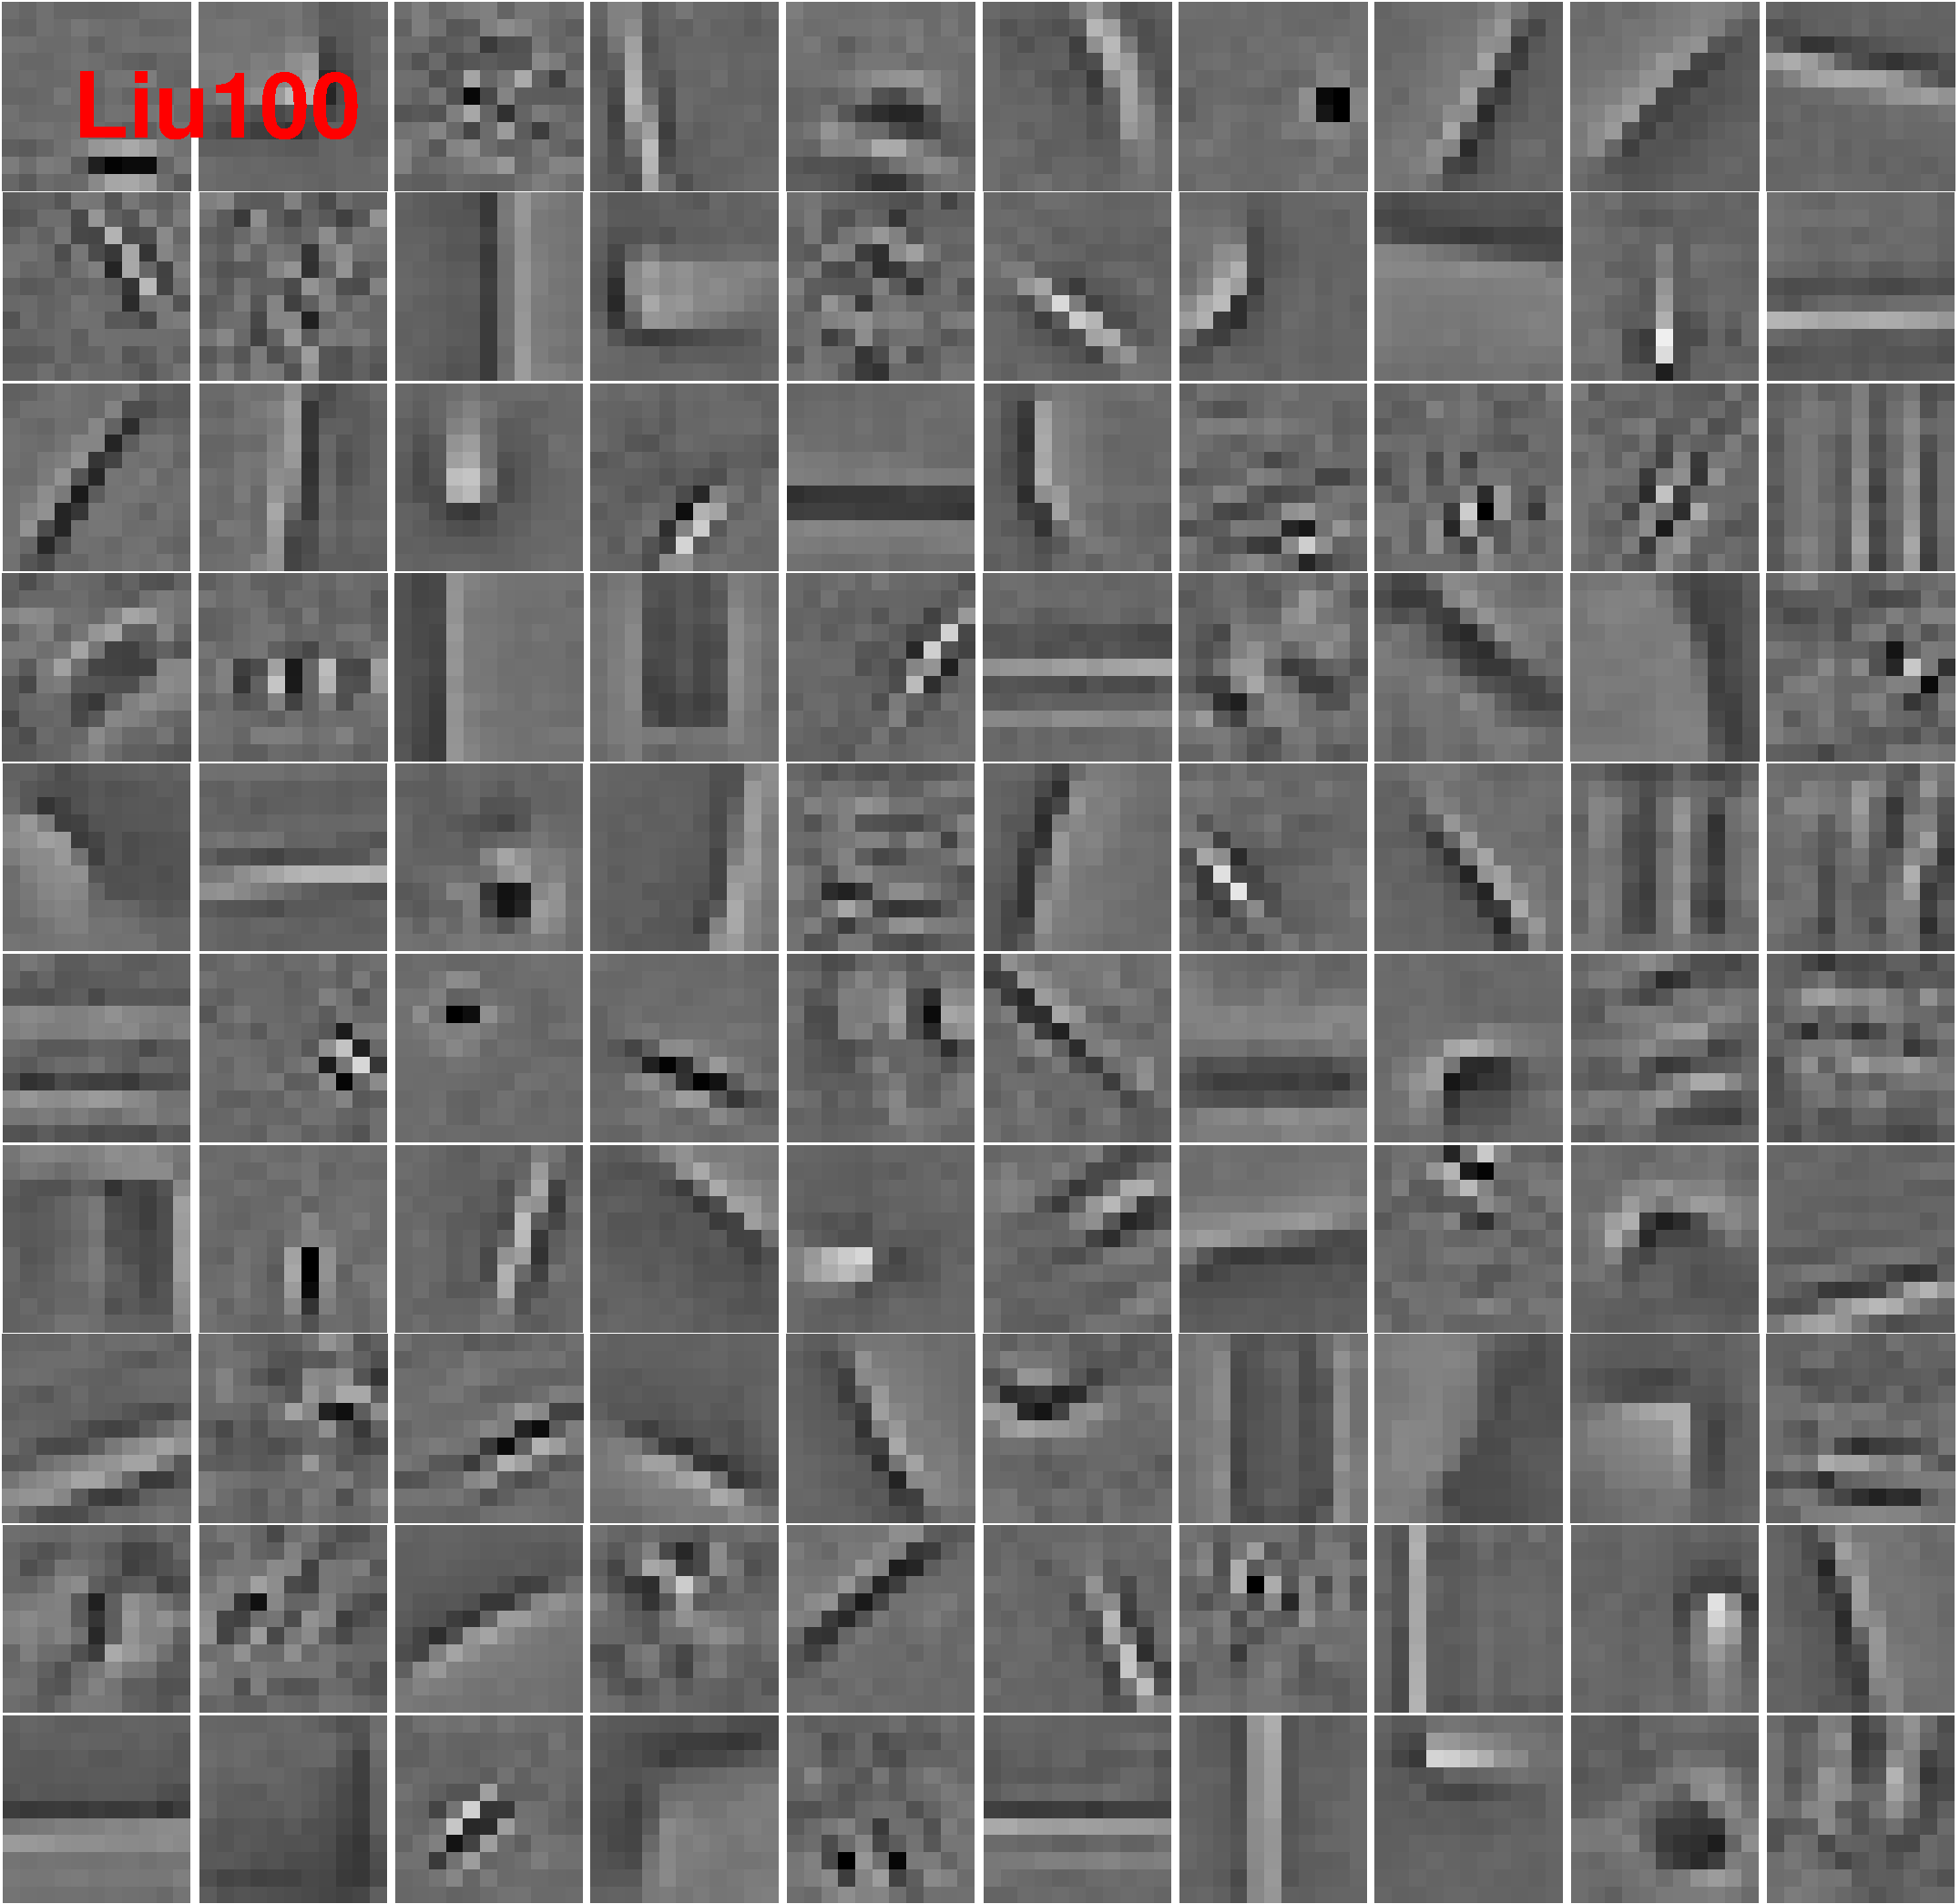
\includegraphics[width=0.6\linewidth]{figure/liu100-filter.pdf}
  \vspace*{2mm}
\end{subfigure}

\begin{subfigure}{1\textwidth}
    \centering
  \includegraphics[width=0.6\linewidth]{figure/online100-filter.pdf}
\end{subfigure}
\end{minipage}
\begin{minipage}{0.5\textwidth}
\centering
\includegraphics[width=1\linewidth]{figure/online400-filter.pdf}
\end{minipage}

\caption{Filters learned from 1000 images by the proposed method and its comparison. (a) The under-complete dictionary ($11 \times 11 \times 100$) learned by~\cite{liu-2018-first}; (b) The under-complete dictionary ($11 \times 11 \times 100$) learned by the proposed method. (c) The over-complete dictionary ($11 \times 11 \times 400$) learned by the proposed method. These under-complete dictionaries, mainly composed of gabor-like filters, can be seen as a subset of the represented over-complete dictionary, which also contains a number of low contrast image features.}
\label{fig:overCompleteDic}
\end{figure}

We demonstrate its capability on 1000 image patches with the size of $100 \times 100$, and learn $11 \times 11 \times 400$ over-complete dictionary, all of which are shown in Fig.~\ref{fig:overCompleteDic} . As a comparison, 100 learned filters by the same algorithm and its comparable approach are also represented for a visual comparison. As can be observed, both of the approaches learn visually similar under-complete dictionaries, while the proposed method shows a $5 \times$ speedup over the other. Furthermore, the learned over-complete dictionary is composed of the gabor-like image features as represented in the under-complete dictionaries, as well as a number of low contrast features which are rarely existed in those under-complete dictionaries. These additional feature information would play an essential role to better represent the natural images, which can be demonstrated in Fig.~\ref{fig:overCompleteDic}. 

There is a bottleneck for under-complete dictionary revealed in the left hand side of fig.~\ref{fig:overComDicAndMinibatch}, that no more apparent progress could be observed when the number of training images is higher than a specific value for both of the online approaches. However, owing to more abundant filters, learning over-complete dictionary overcomes this bottleneck, and it shows a considerable improvement with regard to PSNR to have a sparse representation of the testing images.

{\bfseries Mini-batch.} In practice, the mini-batch strategy would be preferred for a gain of convergence speed, rather than drawing a single sample in each training step. This is also a standard extension to stochastic algorithms. We denote the mini-batch size as $\eta$. In the proposed algorithm, the time complexity for one step dictionary update will not increase linearly with the increase of $\eta$. Concretely speaking, updating $\code$ is implemented by Cholesky decomposition, and one computation of the matrix factorization can be applied to all of the currently selected batches. Herein, the complexity for updating $\eta$ $\code$s at once is cheaper than $\eta$ times the complexity of updating one $\code$. In addition, the time complexity for updating $\filter$ is not affected by the value of $\eta$, which will be executed only once in each training step regardless of $\eta$. One exception is to update surrogate matrices, the complexity of which is $\eta$ linearly dependent, while this is not dominant in the runtime. The results for various mini-batch sizes are shown in Fig.~\ref{fig:overComDicAndMinibatch}. The learned filters are examined on the test set every $2^i$ iterations and the last iteration, where $i=0,1,...$. Note that larger $\eta$ will result in less number of iterations to process all 1000 images. A larger mini-batch size shows a greater progress for first few training steps, though it takes additional running time and memory. Overall, mini-batched updates provides a more runtime efficient learning progress in online-based CSC model, and $\eta=20$ achieves one magnitude speedup to reach a condition with same level convergence.

\begin{figure}[h]
\centering
\begin{subfigure}{0.4\textwidth}
  \includegraphics[width=1\linewidth]{figure/overComplete-ite.pdf}
\end{subfigure} 
\begin{subfigure}{0.55\textwidth}
  \includegraphics[width=1\linewidth]{figure/minibatch.pdf}
\end{subfigure}

\caption{Left: Testing PSNR for the compared method with $K=100$, and the proposed method with $K=100$ and $K=400$, respectively. Every iteration draws a single image from the training dataset. Right: Testing PSNR for the proposed method ($K=400$) with varying values of $\eta$.}
\label{fig:overComDicAndMinibatch}
\end{figure}

\section{Conclusions}
In this work, we present a novel stochastic subsampling strategy for solving the CSC problem in spatial domain. This method significantly improves the runtime performance over the prior frequency-domain solvers, which applies to both batch mode and online-learning mode, as well as generating effective and proven outcomes. The proposed algorithm, for the first time, demonstrates the feasibility that tackling the CSC problem in spatial domain while still holding, or even improving the runtime efficiency. Since the subproblem of updating the code is a highly sparse LASSO, other specific optimization strategies can be applied to further accelerate the computation, for instance the idea proposed in~\cite{johnson2017stingycd}, which solves the LASSO problem by coordinate descent and skips unnecessary updates using the method of safe screening~\cite{ghaoui2012Swfe}. It would be worthy to emphasize that transforming the problem into Fourier domain cannot benefit from these kinds of speedup strategies (including the proposed one). Furthermore, instead of employing uniform subsampling strategy, alternative subsampling strategies can be studied in the future for a gain of learning efficiency, for instance an importance or correlation based sampling strategy which considers the dependency relationship between the signals and the sparse codes.

We have also shown the capability of the developed online algorithm to learn representative and meaningful over-complete dictionary from arbitrary large datasets, and the availability of the dictionary is further verified by the application of image inpainting. It can be foreseen that this capability has widespread applications in the audio and image related tasks, and higher dimensional signal processing. The source code for SBCSC and SOCSC is attached in the supplement for reference. 

{\small
\bibliographystyle{ieee}
\bibliography{egbib}
}

\clearpage
\appendix

%\part*{Supplementary Material\\ Stochastic Convolutional Sparse Coding}

\section{Zooming in on the Filters}

Here we zoom in on the filters from Fig.\ \ref{fig:subsampleResult}. Notice that our filters look more smooth for those Gabor-like filters and also contains less number of noise-like filters.

\begin{figure}[h]
\centering
\begin{subfigure}{0.49\textwidth}
  \includegraphics[width=1\linewidth]{figure/batchFruit100.pdf}
\end{subfigure}
\begin{subfigure}{0.49\textwidth}
  \includegraphics[width=1\linewidth]{figure/heideFruit100.pdf}
  \end{subfigure}
\caption{Zoom-in view of the filters from Figure~\ref{fig:subsampleResult}.}
\end{figure}


\section{Additional Experiments}
In order to show the robustness of the proposed algorithms, We also conduct experiments on city dataset. We first compare SBCSC with the state-of-the-art batch-mode algorithm~\cite{heide2015fast}, and the results are shown in Fig.\ \ref{fig:subsampleResult-city}. Similar to the results shown in Fig.\ \ref{fig:subsampleResult}, SBCSC, with $p=0.1$, outperforms the compared batch-mode algorithm with better outcomes and runtime performance. Since the learning is performed on handful datasets, both of them learn quite a few data-specific image features. The reconstruction quality also shows a shortage of the generalization ability. For example, the eighth image, which contains a large portion of texture information existed in the filters learned from city dataset, can be significantly better reconstructed by such filters compared to those learned from fruit dataset, while it may have poorer performance on other types of images. Furthermore, compared with the over-complete dictionary, we can observe that the presented over-complete dictionary contains both of the image features (superficially similar) appeared in the filters learned from fruit and city dataset, even though they use totally different training images. It also experimentally shows a better reconstruction performance on all kinds of testing images.

\begin{figure}[h]
\begin{subfigure}{0.5\textwidth}
  \includegraphics[width=1\linewidth]{figure/iteVSobj-city.pdf}
\end{subfigure}
\begin{subfigure}{0.5\textwidth}
  \includegraphics[width=1\linewidth]{figure/timeVSobj-city.pdf}
\end{subfigure}

\begin{subfigure}{0.48\textwidth}
  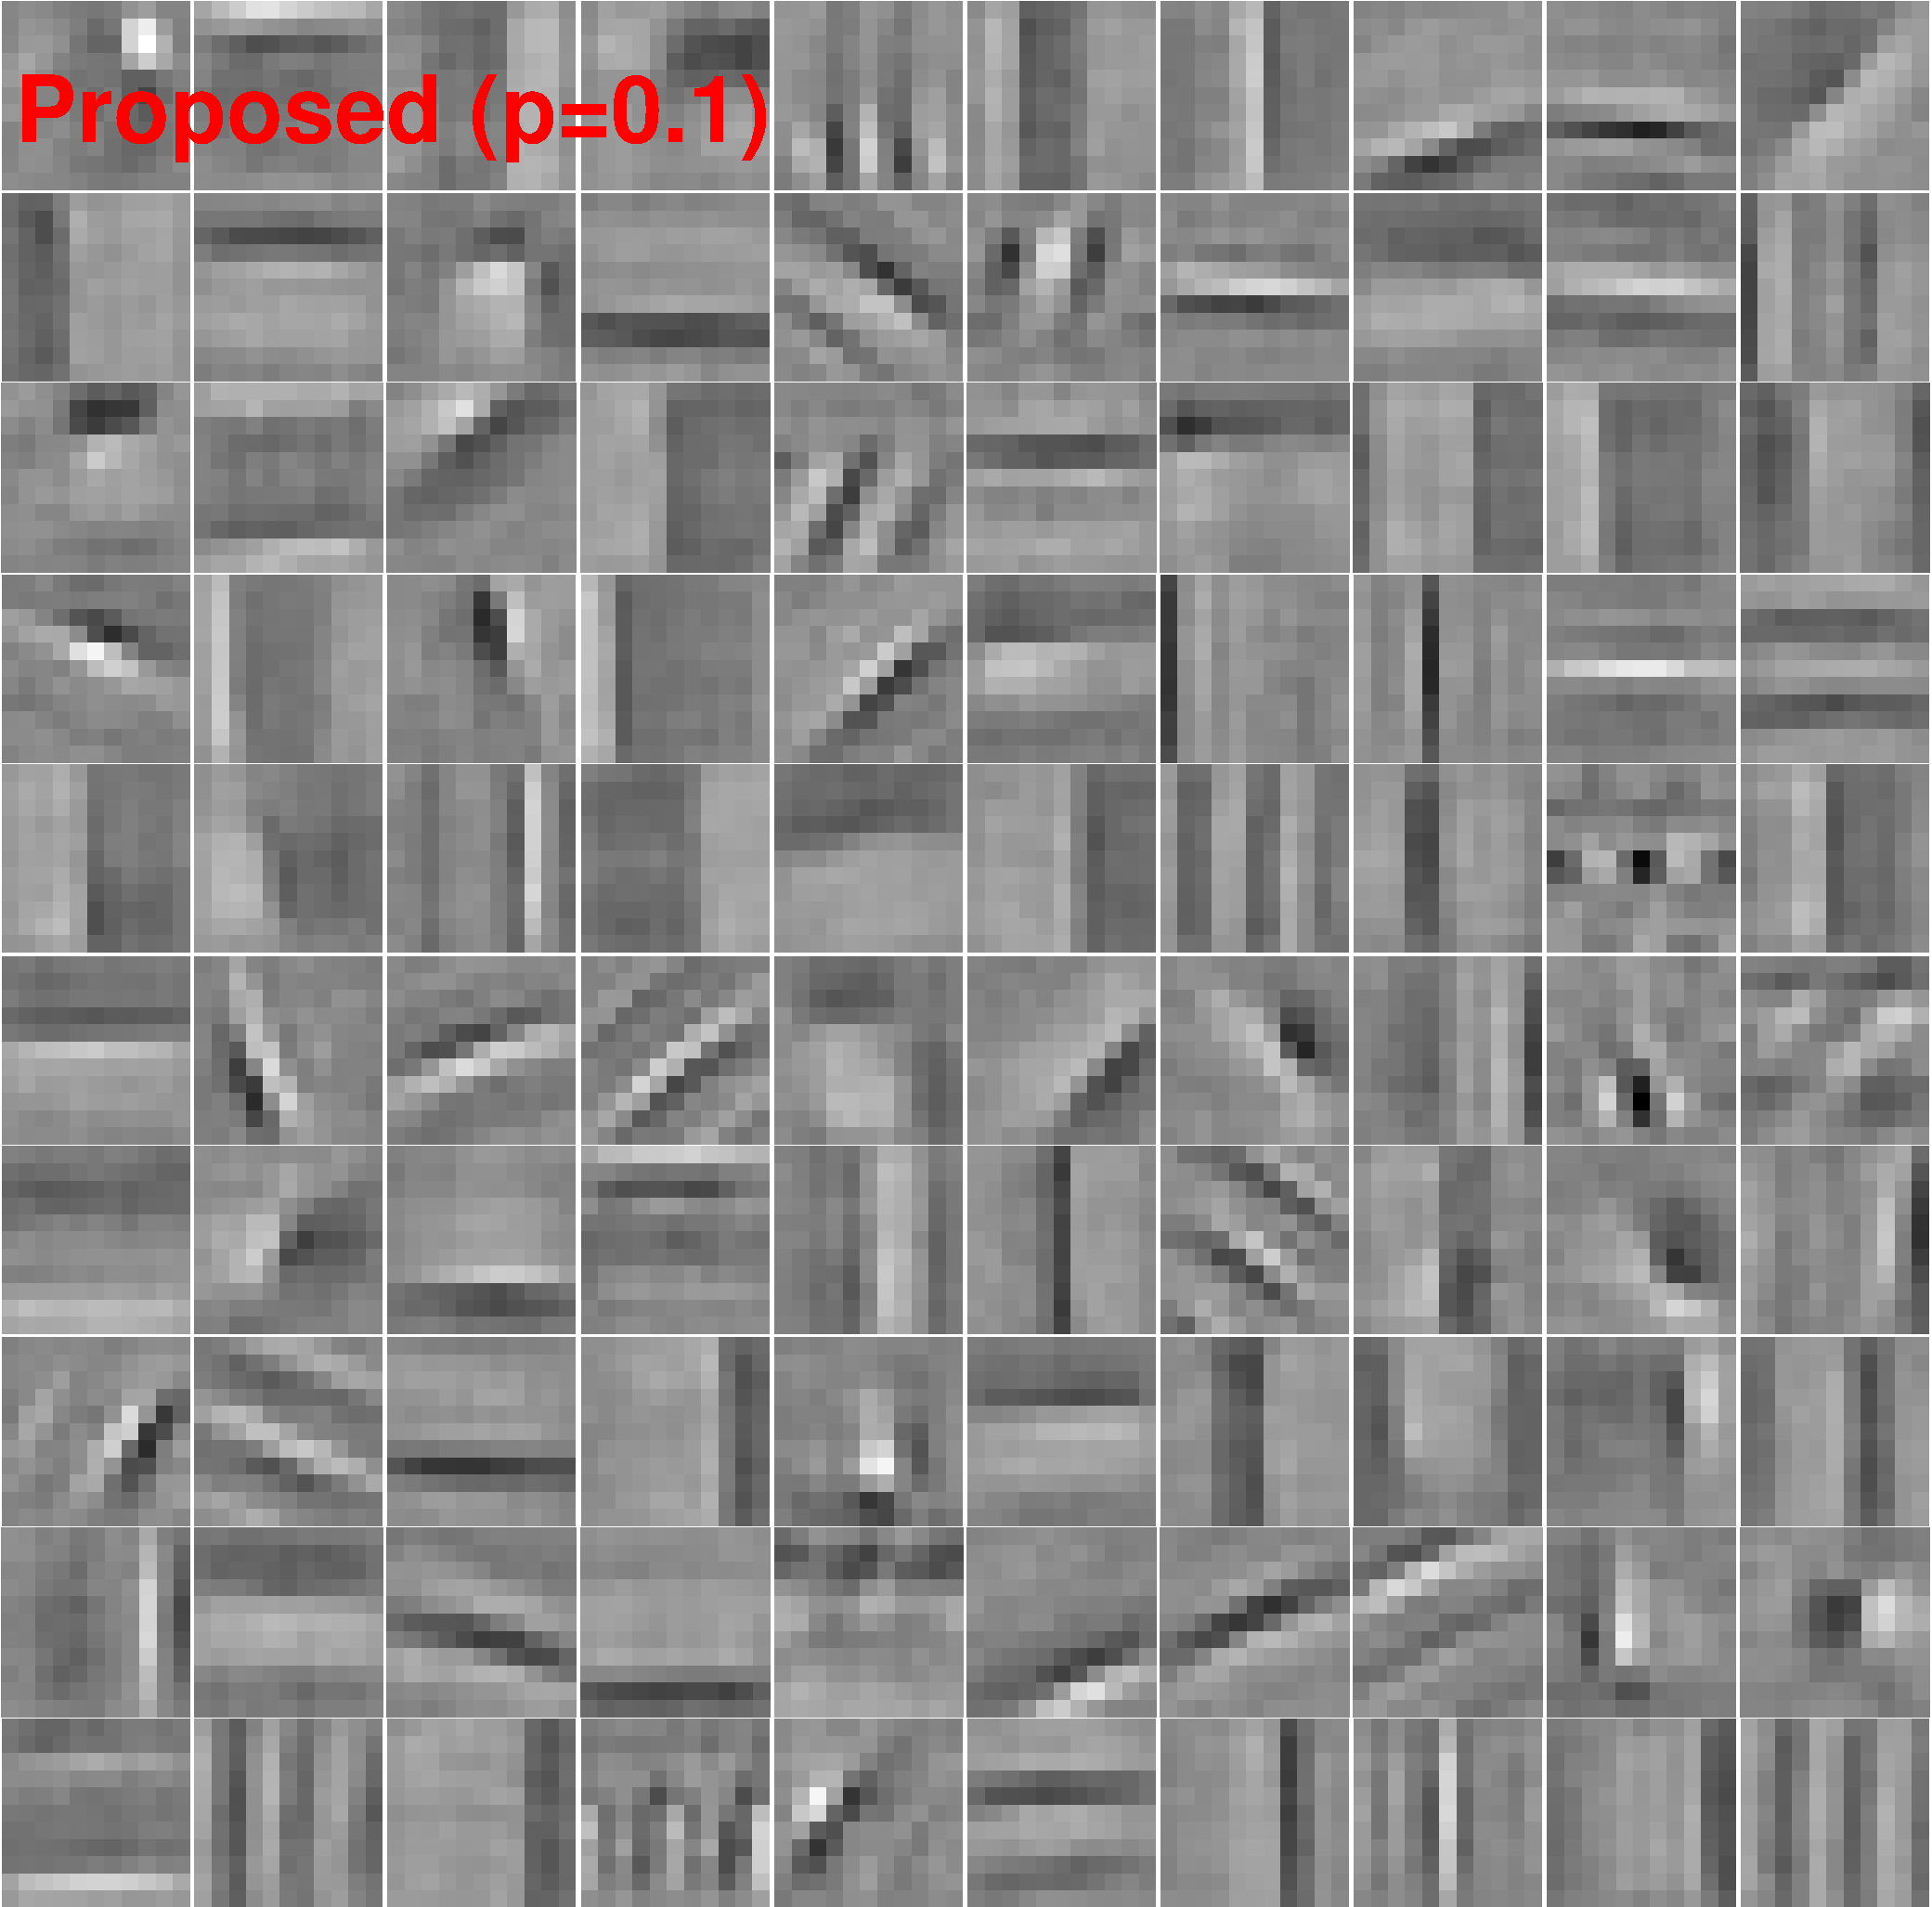
\includegraphics[width=1\linewidth]{figure/batchCity100.pdf}
\end{subfigure}
\begin{subfigure}{0.48\textwidth}
  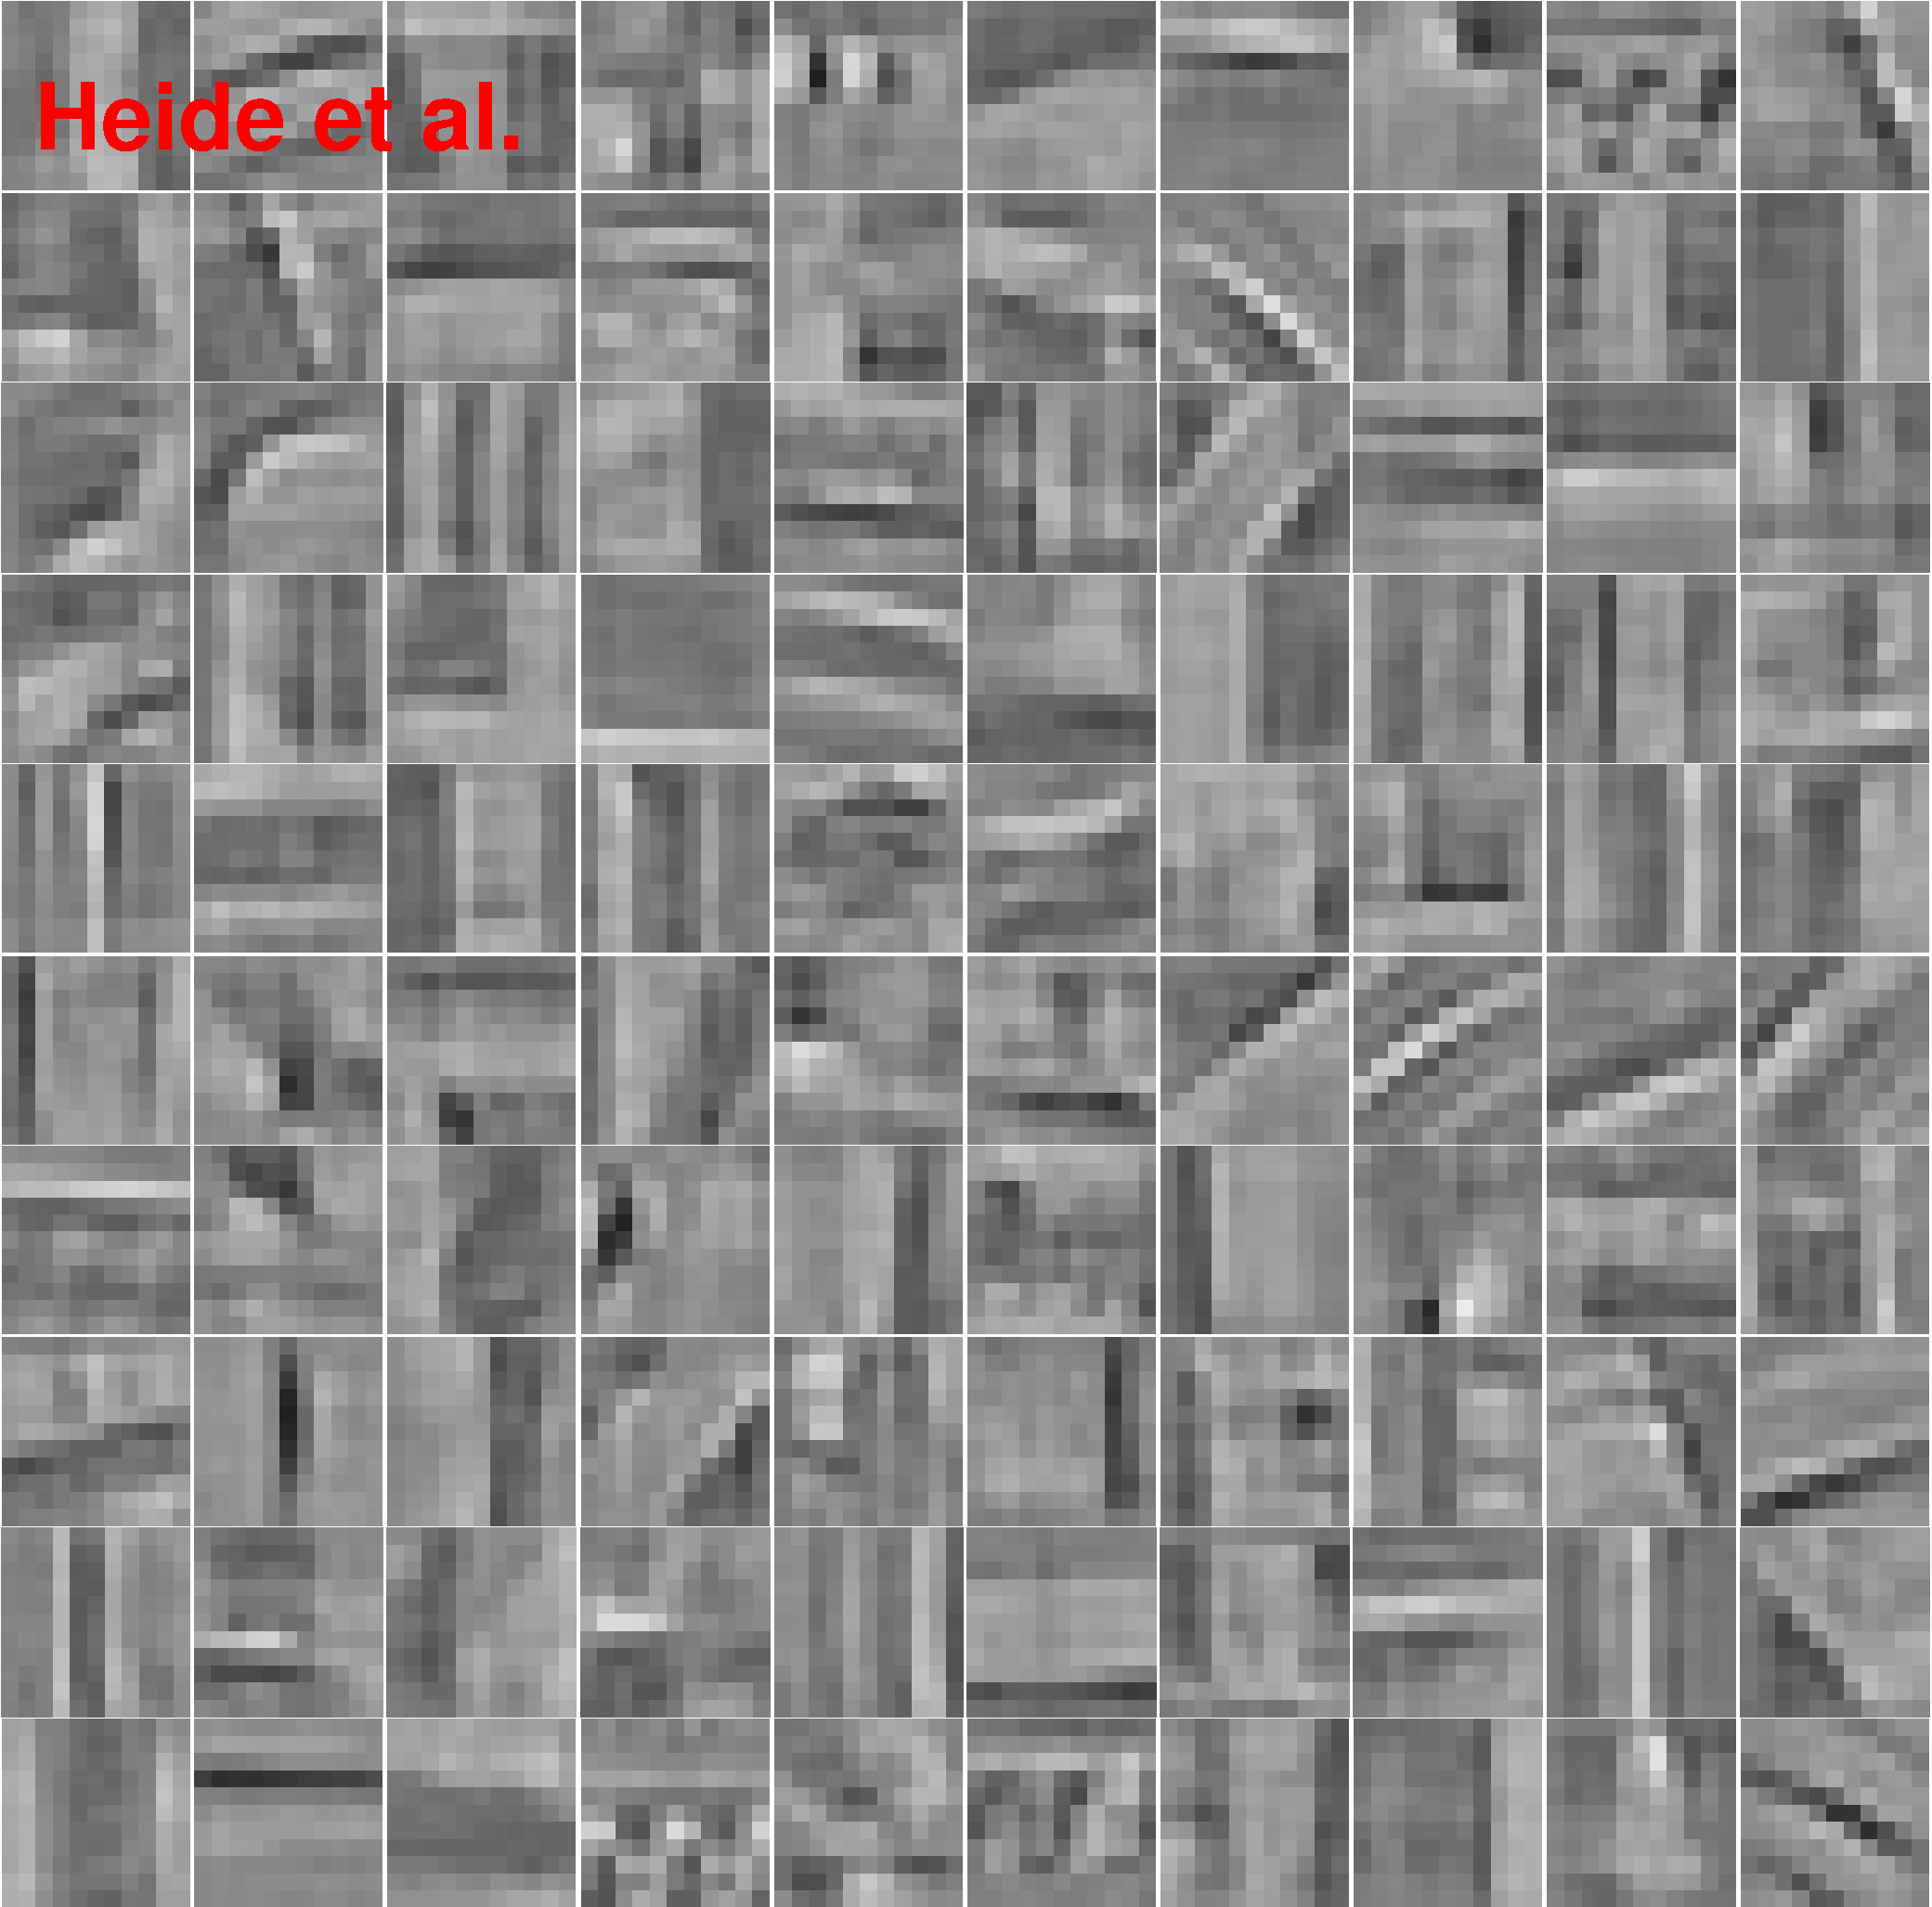
\includegraphics[width=1\linewidth]{figure/heideCity100.pdf}
\end{subfigure}
\vspace{0.2cm}

    \resizebox{1\linewidth}{!}{
        \begin{tabular}{|c||c|c|c|c|c|c|c|c|c|c|}
            \cline{1-11}
            Image & 1 & 2 & 3 & 4 & 5 & 6 & 7 & 8 & 9 & 10 \\
            \hline
            PSNR~\cite{heide2015fast} & 29.67 & \textbf{28.14} & 29.58 & 29.69 & 28.74 & 29.43 & 27.89  & 30.13 & 27.03 & 30.61 \\
            \hline
            PSNR ours & \textbf{29.78} & \textbf{28.14} & \textbf{29.67}  & \textbf{29.85} & \textbf{28.88} & \textbf{29.95} & \textbf{27.97} & \textbf{30.37} & \textbf{27.14} & \textbf{30.89} \\
            \hline
        \end{tabular} }

\caption{Experimental results obtained on the city dataset. Top: Convergence comparison between the-state-of-art batch method~\cite{heide2015fast} and SBCSC with different subsampling probability. Middle: Learned filters by SBCSC with $p=0.1$ and the comparable method. Even though these dictionaries look similar, our method learns more smooth filters. Compared to the learned filters in Fig.\ \ref{fig:subsampleResult}, they have different representations of the dictionaries, where data-specific features are learned from handful training images. Bottom: Numerical comparisons of the reconstruction quality obtained by the presented filters.}
\label{fig:subsampleResult-city}
\end{figure}

We then compare SOCSC with the state-of-the-art online algorithm~\cite{liu-2018-first} on city dataset, the results of which are shown in Fig.\ \ref{fig:onlineSmall-city}. Similar to the results presented in Fig.\ \ref{fig:onlineSmall}, our method obtains comparable outcomes, meanwhile, achieves roughly $5 \times$ speedup.

\begin{figure}[h]
\centering
\begin{subfigure}{0.45\textwidth}
  \includegraphics[width=1\linewidth]{figure/onlineVSliu-ite.pdf}
\end{subfigure}
\begin{subfigure}{0.45\textwidth}
  \includegraphics[width=1\linewidth]{figure/onlineVSliu-time.pdf}
\end{subfigure}

\caption{Experimental results obtained on city dataset. Left: Convergence of the test set objectives for our method (SOCSC) and the state-of-the-art online approach~\cite{liu-2018-first}. Right: Testing PSNR with respect to execution time.}
\label{fig:onlineSmall-city}
\end{figure}

\section{Over-complete Dictionary and Large Datasets}
In this section, we verify the importance of a large dataset when learning the over-complete dictionary. in Fig.~\ref{fig:overCompleteDic-dataset}, we show a visual and quantitative comparisons between the over-complete dictionaries respectively learned by batch-mode algorithm on small dataset (the fruit dataset) and online-mode algorithm on large dataset (1000 images). Most of the filters learned from small dataset have poor structures and reveal very limited representative ability. The numerical results also demonstrate that it even shows a degraded reconstruction performance compared to the under-complete dictionary. Owing to plentiful training samples, our over-complete dictionary not only shows visually decent structures and more representative image features, but also leads to a significant improvement on image reconstruction. Based on all experimental results, it implies that the number of filters and number of training samples are both essential in the CSC model, therefore, the proposed algorithm has prominent advantages over the existing approaches.

\begin{figure}[h]
\centering
  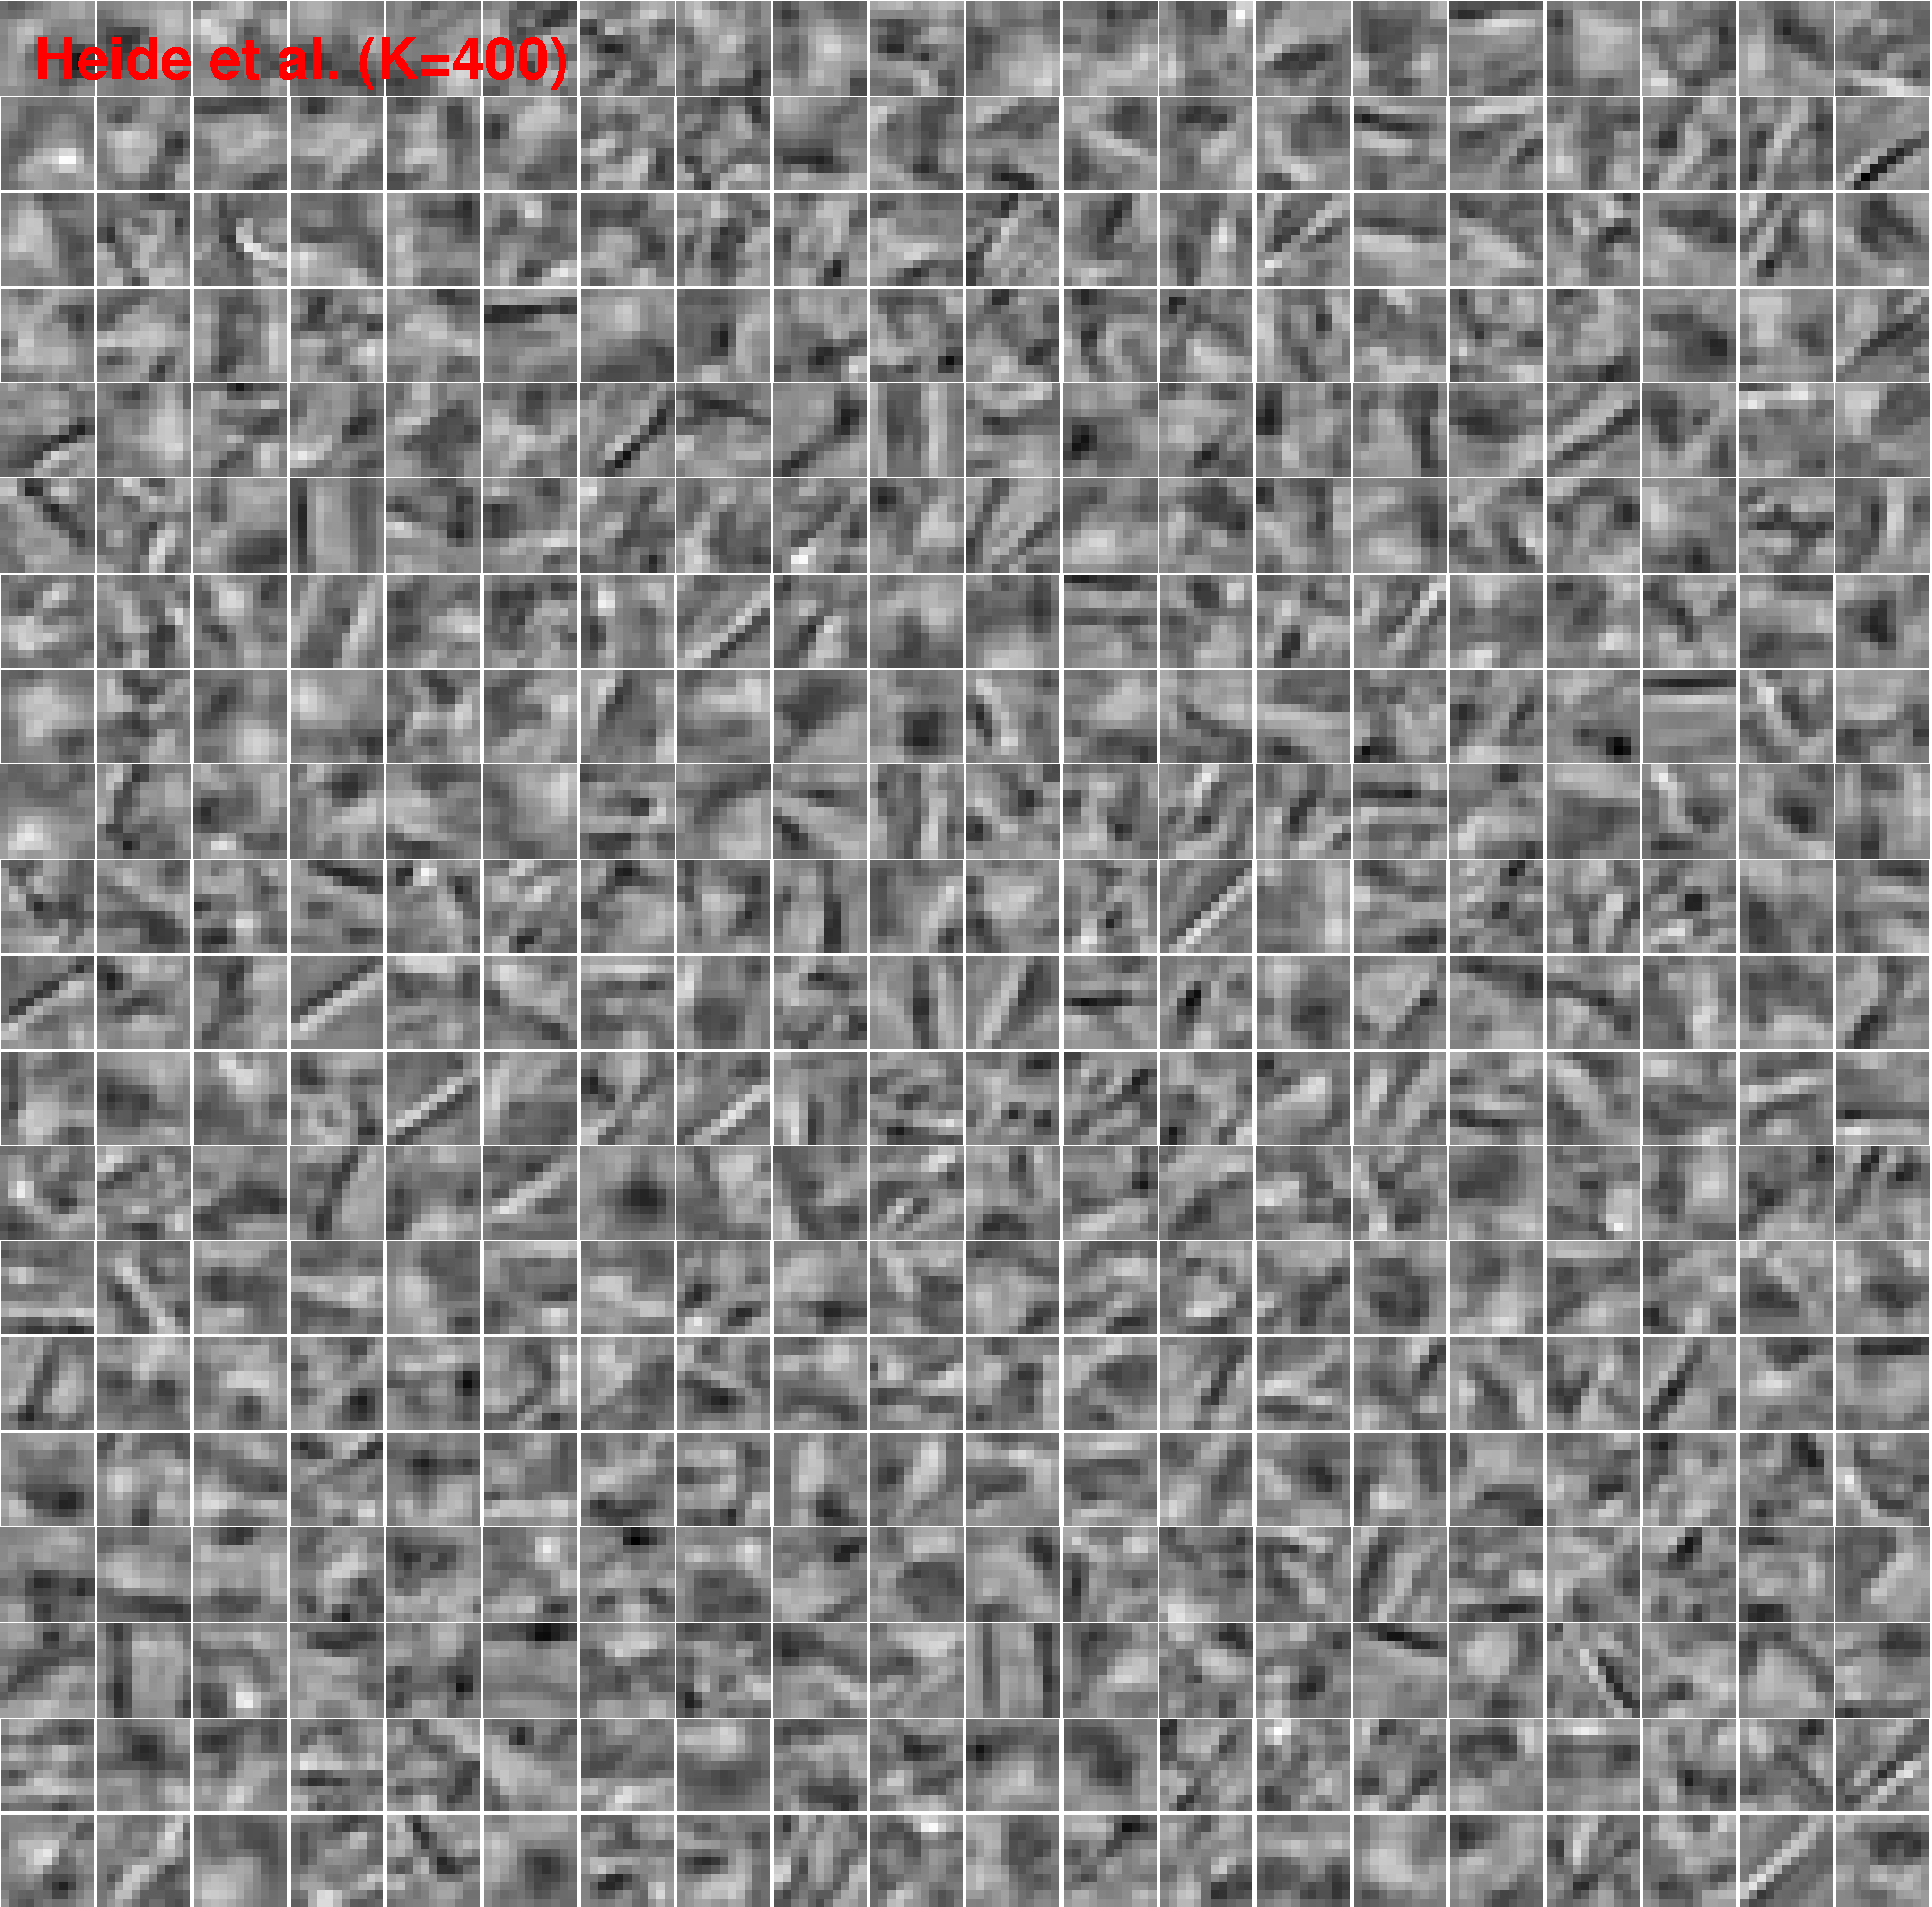
\includegraphics[width=0.7\linewidth]{figure/heide400-supple.pdf}
  \includegraphics[width=0.7\linewidth]{figure/online400-supple.pdf}
  \vspace{0.2cm}

    \resizebox{1\linewidth}{!}{
        \begin{tabular}{|c||c|c|c|c|c|c|c|c|c|c|}
            \cline{1-11}
            Image & 1 & 2 & 3 & 4 & 5 & 6 & 7 & 8 & 9 & 10 \\
            \hline
            PSNR~\cite{heide2015fast} & 29.60 & 28.11 & 29.47 & 28.98 & 28.79 & 29.21 & 28.03  & 29.31 & 27.42 & 30.52 \\
            \hline
            PSNR ours & \textbf{30.24} & \textbf{28.34} & \textbf{29.95}  & \textbf{30.30} & \textbf{29.43} & \textbf{29.96} & \textbf{28.24} & \textbf{30.57} & \textbf{27.72} & \textbf{31.67} \\
            \hline
        \end{tabular} }
  \caption{ Visual and numerical comparisons between the learned over-complete dictionaries by batch-mode algorithm and by online-mode algorithm. Top: Over-complete dictionary learned by batch CSC model~\cite{heide2015fast} on small dataset, and proposed online CSC model (SOCSC) on large dataset. Bottom: Respective reconstruction quality for these two over-complete dictionaries.}
  \label{fig:overCompleteDic-dataset}
\end{figure} 

\end{document}
